\chapter{Data Collection and Processing}
\label{chap:data_processing}
\setlength{\parskip}{1em}

\section{Input Vectors and Modalities}
To accurately map to the highly decoupled workflows of contemporary university students, the Lectura ecosystem was architected to aggressively ingest multiple disparate data vectors. Because modern academia fundamentally rejects singular transmission formats, the ingestion engine is decoupled from the generative engine, allowing seamless processing of the following input streams:

\begin{itemize}[label=\textendash]
    \item \textit{YouTube Video Transcripts:} The primary vector for mass-distributed educational content. Lectura programmatically hooks into localized API endpoints to extract closed-captions, intercepting the raw spoken narrative of digital lectures before it encounters manual transcription bottlenecks.
    \item \textit{Spatial Document Uploads:} Handling the ubiquitous necessity of PDF, DOCX, and raw TXT documentation, encompassing everything from heavily formatted, multi-column research papers to bare-bones digital textbook chapters.
    \item \textit{Raw Text Input:} Bypassing the file-upload overhead entirely, the interface permits users to directly inject clipboard data, an essential pathway for fragmented forum posts or highly localized instructor emails.
    \item \textit{Future Audio-Derived Telemetry:} Architectural considerations have been coded to eventually support direct WebSocket-streamed audio (Speech-to-Text), targeting the capture of live, synchronous classroom lectures.
\end{itemize}

This robust extraction capability directly addresses Objective 1 stated in the Introduction, which mandates the creation of multimodal ingestion pipelines capable of handling YouTube URLs and local documents without friction.

\section{Multimedia Transcript Sanitization}
Scraping raw analytical data from a YouTube endpointcopy invariably yields highly contaminated strings. The raw schema delivered by the YouTube Data API is severely adulterated with HTML artifacts (e.g., \verb|&amp;|, \verb|&quot;|), embedded timestamps, auditory non-speech markers ([Applause], [Music]), and profoundly fragmented sentence structures caused by auto-generated captioning cadence.

If this contaminated payload is fed directly into a Large Language Model, the prompt coherence degrades catastrophically, prompting hallucinatory outputs. Consequently, the Lectura backend dictates a severe pre-processing gauntlet.

First, a regular expression (regex) engine aggressively scrubs HTML residuals and isolates out non-verbal acoustic markers. Second, the algorithm mathematically addresses the structural fragmentation. By calculating the delta between absolute timestamps, the engine defines a hard ``paragraph break'' whenever a temporal gap exceeds 3.0 seconds. This logical grouping synthesizes a naturally flowing narrative from a heavily fractured VTT/SRT file. This resulting artifact is categorically superior for downstream LLM evaluation because it preserves the semantic proximity of related concepts.

\subsection{Visual Content Extraction from Video Frames}
One limitation of processing videos using only transcripts is that it relies entirely on what is spoken aloud. Educational videos often include important information on the screen, such as slide titles, math formulas, code snippets, or diagrams. If the instructor does not read this text out loud, it will be missing from the final transcript.

To solve this problem, Lectura includes an optional feature to extract visual content. When a user selects the "Read text on video screen" option, the backend sends the video frames to the Google Gemini multimodal API along with the audio transcript. The model uses Optical Character Recognition (OCR) to read the text that appears on the screen.

This extracted text is then added to the prompt as extra context. The system is instructed to use the on-screen text as additional evidence and to prioritize it if there is a conflict between the subtitles and the visual text. This approach helps ensure that the generated summaries and flashcards contain a more complete representation of the lecture. 

This feature is especially useful for technical subjects where instructors often write formulas on a board without reading every variable aloud. By extracting the text directly from the frames, the generated study materials can include these specific details. By mathematically sanitizing transcripts and implementing OCR extraction, this methodology directly addresses Objective 2, ensuring that algorithmic cleaning protocols yield high-fidelity text strings for subsequent LLM processing.

\section{Heuristic Document Extraction}
Conversely, PDF extraction presents an entirely divergent engineering hurdle: spatial obfuscation. PDF files inherently lack underlying semantic structure; they are merely mathematically rendered coordinates mapping glyphs onto a digital canvas. A multi-column academic paper, if parsed linearly by file bytes, will violently mix the leftmost paragraph with the rightmost paragraph, destroying the intellectual payload.

Lectura circumvents this utilizing advanced spatial heuristics (primarily leveraging the \texttt{pdfplumber} engine via Python microservices or equivalent Go libraries). The processing loop dissects the document matrix, analyzing the absolute x, y coordinates of discrete character blocks. It calculates localized bounding boxes, thereby differentiating a structural header from a primary text column. Elements mathematically recognized as page numbers, repeating footers, or marginalia are programmatically excised. Multi-column documents are sequentially sorted by their horizontal vectors, guaranteeing that the final serialized text stream perfectly mirrors the organic, top-to-bottom optical reading flow of a human user. Similar to video processing, this heuristic mapping directly aligns with Objective 1 by ensuring spatial PDFs are successfully transformed into structured input arrays.

\section{Prompt Engineering and Context Window Dynamics}
Once the data vector is unified into a sanitized, serialized string, it crosses the boundary into the Generative AI layer. Modern contextual models, while vast, maintain absolute token limits. Delivering a 4-hour semantic transcript directly into a single API call risks out-of-memory errors or severe truncation.

Lectura employs ``Mathematical Contextual Chunking with Sliding Overlaps.'' If the payload breaches a defined maximum token threshold ($T_{\max}$), the text is partitioned into sequential arrays $C = \{c_1, c_2, \dots, c_k\}$, deliberately overlapping each chunk by $O_{\text{lap}}$ tokens to mathematically ensure that complex concepts bridging two boundaries are not abruptly severed. The total number of chunks $k$ derived from a source text of length $L$ is roughly bounded by:


\begin{equation}
    k = \left\lceil \frac{L - O_{\text{lap}}}{T_{\max} - O_{\text{lap}}} \right\rceil
\end{equation}

To rigorously enforce this protective overlapping logic across the backend processors before data hits the external LLM boundary, the ingestion engine executes the precise deterministic parsing sequence documented in Algorithm~\ref{alg:sliding_window}.

\begin{algorithm}[htbp]
\caption{Sliding Window Context Overlap Extraction}
\label{alg:sliding_window}
\begin{algorithmic}[1]
    \REQUIRE Extracted, monolithic string $S$; Max token limit $T$; Overlap integer $O$
    \ENSURE Array of discrete context chunks $C$
    
    \STATE $\textit{tokens} \leftarrow \text{Tokenize}(S)$
    \STATE $L \leftarrow \text{Length}(\textit{tokens})$
    \STATE $C \leftarrow [ ]$
    \STATE $\textit{index} \leftarrow 0$
    
    \WHILE{$\textit{index} < L$}
        \STATE $\textit{end\_boundary} \leftarrow \min(\textit{index} + T, L)$
        \STATE $\textit{chunk} \leftarrow \textit{tokens}[\textit{index} \dots \textit{end\_boundary}]$
        \STATE $C\text{.append}(\textit{chunk})$
        
        \IF{$\textit{end\_boundary} == L$}
            \STATE \textbf{break}
        \ENDIF
        
        \STATE $\textit{index} \leftarrow \textit{index} + T - O$ \COMMENT{Shift backward by $O$ to retain context}
    \ENDWHILE
    
    \RETURN $C$
\end{algorithmic}
\end{algorithm}


These processed sub-arrays are subsequently bonded to ``System Prompt Directives.'' Rather than allowing the LLM to dynamically determine its persona, the system forcibly injects predefined constraint headers into every chunk $c_n$. For example, the summary heuristic dictates: ``You are an elite academic structuralist. Parse the trailing context and export it strictly formatted as Markdown Cornell notes.'' This deterministic bounding guarantees that the output satisfies rigid pedagogical criteria without memory-loss.

\subsection{Visual Rhythm and Strict JSON Arrays}
The generation of presentation slides introduces the most computationally brittle prompting requirement. To achieve the ``True Gamma Standard'' aesthetic, the prompt cannot simply ask for ``a presentation.'' Instead, it enforces a strict JSON schema array detailing distinct, rigid slide typologies. The Gemini LLM is categorically constrained to return an array of objects where each object possesses a \texttt{slide\_type} enumerated from a strict list (e.g., \texttt{hero\_image}, \texttt{big\_stat}, \texttt{icon\_grid}, \texttt{two\_column}).

Furthermore, the prompt forces severe string-length penalties to eliminate the ``wall of text'' phenomenon common in legacy slide generators. It dictates that an \texttt{icon\_grid} slide must contain exactly three or four semantic bullet points, none exceeding eight words. This aggressive prompt sculpting surgically extracts the core narrative and perfectly formats the data payload for immediate rendering within the React presentation framework. Through strict contextual chunking and JSON schema enforcement, this architecture directly fulfills Objective 3 (Generative Summarization) and Objective 4 (Visual Presentation Genesis) by guaranteeing structurally consistent, predictable outputs from the language model.

\section{Output Validation and Persistence Topology}
Generative processing is inherently volatile. An API might occasionally fail to adhere to structural delimiters (e.g., abandoning the required \texttt{Question:} and \texttt{Answer:} prefixes mid-way through a flashcard generation loop). To counteract this, Lectura invokes a secondary validation mechanism before persisting any data.

The Go backend employs string-matching and JSON-schema validation to audit the returned payload. If an LLM response violates format parameters, the worker node triggers an autonomous retry mechanism utilizing an aggressively corrective secondary prompt. Furthermore, to eliminate vector-based Cross-Site Scripting (XSS) attacks injected through parsed media, aggressive multi-layer assignment sanitization strips errant inline scripts before the data hits the database.

Upon validation, the telemetry is normalized into the PostgreSQL relational framework. User identities and credentials remain highly isolated, while the core payload is distributed across Content (the heavily cleansed transcript source), Artifacts (the LLM-generated JSON permutations of quizzes, summaries, presentations, and flashcards), and Interactions (the longitudinal behavioral metrics tracking quiz velocity and recall accuracy). This strict normalization and storage hierarchy directly addresses Objective 8 from the Introduction, successfully establishing the analytics and persistence layer required to log student performance over time.

\section{Extraction Pipeline Representation}
The deterministic progression from chaotic exterior multimedia to surgically refined relational database entries is visually codified within the pipeline schema depicted in Figure~\ref{fig:pipeline}.

\begin{figure}[htbp]
\centering
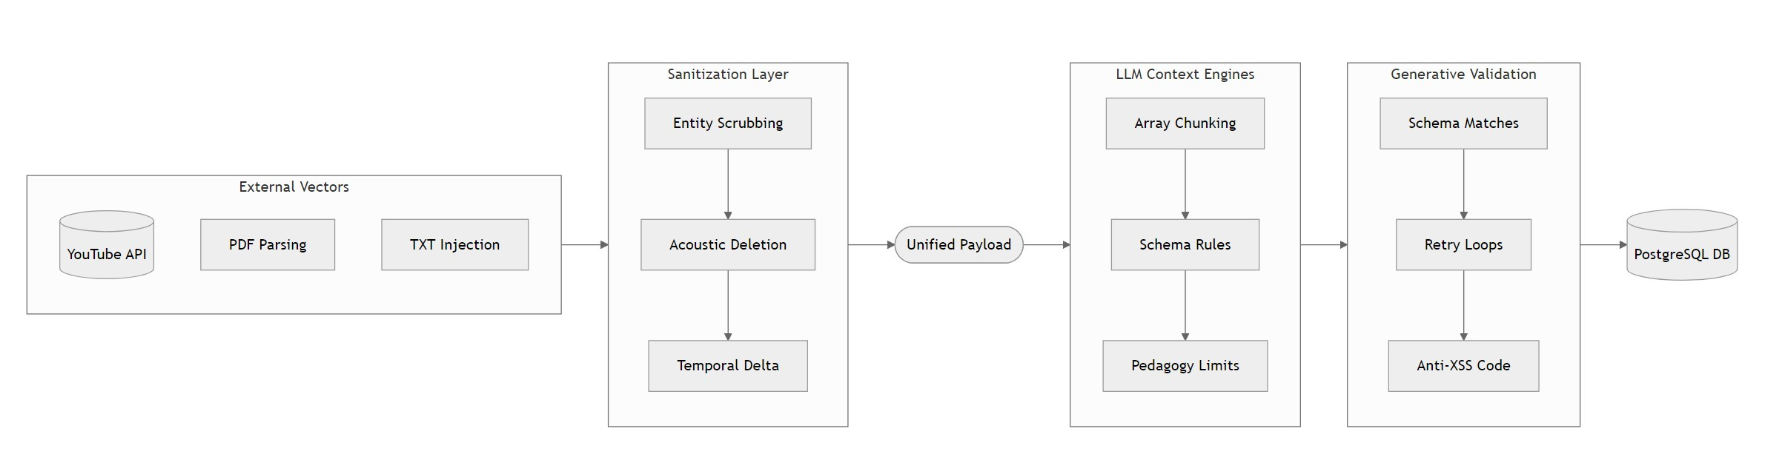
\includegraphics[width=\textwidth]{chapters/chapter03/images/figure3.png}
\caption{Semantic representation of the data ingestion and generative validation pipeline.}
\label{fig:pipeline}
\end{figure}